% \begin{notation}[label={not:OpsFS}]{Notation for variables in the current section}
%     In this section, we use the variable \( x \) to represent time and \( y \) to represent distance.
%   \end{notation}

The notions of union and intersection in fuzzy sets were first introduced by Zadeh \cite{Zadeh1965} using the operations $\max\{A(x),B(x)\}$ and $\min\{A(x),B(x)\}$ respectively. These can be intuitively interpreted as follows: the union is the \textit{smallest} fuzzy set (having lowest membership values) that contains both sets, while the intersection is the \textit{biggest} fuzzy set (having highest membership values) that is contained by both sets.\\

However, these operations can be generalized by two broader classes of operators: triangular norms (for intersection) and triangular conorms (for union).

Triangular norms were first introduced by Karl Menger in 1942 \cite{OriginTNorms} in the context of probabilistic metric spaces. When generalizing distances between points to probability distributions (representing the probability that the distance is less than or equal to a given value), Menger defined an operation $T:\,[0,1]\times [0,1]\to [0,1]$ to preserve the triangular inequality. For points $x,y,z$ in a metric space with distance function $d(\cdot,\cdot)$, this operation satisfies:

\begin{equation}\label{eq:Ftriangle_inequality}
d(x, z) \leq d(x, y) + d(y, z) \quad \longrightarrow \quad F_{xz}(t + s) \geq T(F_{xy}(t), F_{yz}(s)) \quad \forall t,s \geq 0
\end{equation}

This inequality means that the probability of $d(x,z)$ being less than $t+s$ must be at least the t-norm of the probabilities that $d(x,y)<t$ and $d(y,z)<s$. Note the change from $\leq$ to $\geq$ in the inequality. This is consistent with \textit{larger} probabilities indicating \textit{smaller} distances are more likely.\\

Since this originated in the context of distances, the following properties were required for an operator to be a t-norm\footnote{Associativity and one identity were not originally proposed by Menger but were later added by Sklar and Schweizer \cite{Sklar1983} in their refinement of triangular norms}:

\begin{itemize}
  \item \textbf{Symmetry:} The order of combining probabilities shouldn't matter, just as intersection of sets is commutative. That is, combining probabilities for distances $(x,y)$ and $(y,z)$ should give the same result regardless of order.
  
  \item \textbf{Associativity:} When combining multiple probabilities (e.g., for paths through points $x,y,z,w$), the grouping shouldn't affect the result. This extends the triangular norm to be consistent with polygonal inequalities, similar to how nested intersections satisfy $(A \cap B) \cap C = A \cap (B \cap C)$.
  
  \item \textbf{Monotonicity:} If the probability $F_{xy}(t)$ increases, then the lower bound for $F_{xz}(t+s)$ given by $T(F_{xy}(t), F_{yz}(s))$ should not decrease. This is analogous to how adding elements in crisp sets (or increasing membership degrees in fuzzy sets) cannot reduce the intersection set.
  
  \item \textbf{One Identity:} If $F_{yz}(s) = 1$ (meaning $d(y,z) < s$ with certainty), then $F_{xz}(t+s)$ depends only on $F_{xy}(t)$. This is analogous to how intersecting with the universal set preserves the original set.
\end{itemize}


% \say{The name \textit{triangular norm} refers to the fact that in the framework of probabilistic metric spaces, t-norms and t-conorms are used to generalize triangle inequality of ordinary metric spaces.}\cite{NGAN2018}\\

Therefore, the concept of intersection (conjunction) of fuzzy sets is generally represented by a triangular norm (also called a t-norm).

\begin{definition}[Triangular Norm]
    A mapping $T:[0,1]\times [0,1] \longrightarrow [0,1]$ that satisfies:
    \begin{romanenum}
      \item \textbf{Symmetricity:} $T(x,y) = T(y,x) \quad \oldforall x,y \in [0,1]$
      \item \textbf{Associativity:} $T(x,T(y,z)) = T(T(x,y),z) \quad \oldforall x,y,z \in [0,1]$
      \item \textbf{Monotonicity:} $T(x,y) \leq T(x',y') \quad \textnormal{if }x\leq x' \textnormal{ and } y\leq y' \quad \oldforall x,y,x',y' \in [0,1]$
      \item \textbf{One Identity:} $T(x,1) = T(1,x) = x \quad \oldforall x \in [0,1]$
    \end{romanenum}
    is called a triangular norm or t-norm. Defines the \textbf{intersection} of two fuzzy sets $A$ and $B$ on $X$ by giving the membership function as $(A \cap B) (x) = T(A(x),B(x)) \forall x \in X$ 
\end{definition}

Its dual operator can also be obtained by a similar reasoning as before, but instead of considering the probability distribution of finding both points closer than a given distance, it considers the probability distribution ($G_{uv}(t) = 1 - F_{uv}(t)$) of finding them further apart than that distance. In this case, both inequalities are $\leq$ since larger probabilities indicate that greater distances are more likely.
\begin{equation}\label{eq:Gtriangle_inequality}
d(x, z) \leq d(x, y) + d(y, z) \quad \longrightarrow \quad G_{xz}(t + s) \leq S(G_{xy}(t), G_{yz}(s))
\end{equation}

The reasoning regarding the properties is entirely analogous to the previous case, with the only difference being that $F_{uv}(t) = 1 \Leftrightarrow  G_{uv}(t) = 0$, and here the identity element is zero (union with the empty set).



\begin{definition}[Triangular Conorm]
  A mapping $S:[0,1]\times [0,1] \longrightarrow [0,1]$ that satisfies:
  \begin{enumerate}[(i)]\setlength{\itemindent}{2em}
    \item \textbf{Symmetricity:} $S(x,y) = S(y,x) \quad \oldforall x,y \in [0,1]$
    \item \textbf{Associativity:} $S(x,S(y,z)) = S(S(x,y),z) \quad \oldforall x,y,z \in [0,1]$
    \item \textbf{Monotonicity:} $S(x,y) \leq S(x',y') \quad \textnormal{if }x\leq x' \textnormal{ and } y\leq y' \quad \oldforall x,y,x',y' \in [0,1]$
    \item \textbf{Zero Identity:} $S(x,0) = S(0,x) = x \quad \oldforall x \in [0,1]$
  \end{enumerate}
  is called a triangular conorm or t-conorm. Defines the \textbf{union} of two fuzzy sets $A$ and $B$ on $X$ by giving the membership function as $(A \cup  B) (x) = S(A(x),B(x)) \forall x \in X$ 
    
\end{definition}

Complement was defined by Zadeh \cite{Zadeh1965} as\footnote{This is not the only definition that satisfies the axioms of a complement and is compatible with the classical limit, but it is the simplest one and will be used in this text. Other alternatives and their axioms can be found in \cite{Sladoje2007}. In \cite{Klement2000}, this is called the standard negation $N_s$.}:

\begin{definition}[Complement]
  The complement of a fuzzy set $A\in \fuzzy{X}$ is another fuzzy set with membership function given by $\overline{A}(x) \coleq 1 - A(x) \forall x\in X$
\end{definition}

Notice that this definition of complement is consistent with the classical definition of complement but implies that an element might have \textbf{non-zero partial membership} to both a fuzzy set and its complement: Let $A$ be a fuzzy set on $X$ and $x \in X / A(x)\notin \{0,1\}$ then $\overline{ A}(x)= 1 - A(x) \notin \{0,1\}$.\\

One consequence of this fact is that the union of a fuzzy set and its complement is not the total set in general. Analogously, the intersection will not the empty set in general. Those two properties that hold in classical sets but might not be true in fuzzy sets, are often called the \textbf{laws of excluded middle and of non-contradiction}, respectively.\\

However, there are t-norms and t-conorms such as the ones named after \luka that do satisfy both laws\footnote{Indeed, all continuous t-norms in agreement with non-contradiction are isomorphic to \luka \cite[p.~7]{LukasiewiczNonContrad}.}. Another example is the drastic t-norm which also satisfies the law of non-contradiction, but not the law of excluded middle. See example \ref{ex:basic_tnorms} for their formal expressions. \signal{All of this, has implications for the derived logic that will be explained in section \ref{sec:fuzzy_logic}. }\\

Another important property that classical union and intersection satisfy is De Morgan's Laws. For an arbitrary pair of t-norm and t-conorm, these laws are not automatically satisfied. However, there are specific pairs that do fulfill them. To illustrate the relationship between t-norms and t-conorms that satisfy De Morgan's Laws, we can use our probabilistic metric space analogy. Reconsidering the probabilistic metrics $F,G$ introduced earlier and substituting $F = 1 - G$ into equation \ref{eq:Ftriangle_inequality}, we obtain:

\[ G_{xz}(t + s) \leq 1 - T(1 - G_{xy}(t), 1 - G_{yz}(s))\]

Comparing this with equation \ref{eq:Gtriangle_inequality}, we can derive a relationship between t-norms and t-conorms\footnote{The relation from proposition \ref{prop:rel_tnorm_tconorm} directly mirrors the classical set union definition via intersection and negation ($A\cup B \coleq \neg (\neg A \cap \neg B)$), which can be visualized with a Venn diagram. Therefore, it is natural that this condition is equivalent to the De Morgan's Laws.}, which is formalized in the following proposition:

\begin{proposition}[Relationship between t-norm and t-conorm]\label{prop:rel_tnorm_tconorm}
  Given a t-norm $T$, the t-conorm is $S(a,b)\coleq 1 - T(1-a, 1-b)$ if and only if the union and intersection defined by that pair satisfy the De Morgan's Laws.
\end{proposition}
\begin{remark}
  It is easy to see that the previous relation is equivalent to $T(a,b) = 1-S(1-a, 1-b)$ which can be obtained simply by substituting $a'=1-a$ and $b'=1-b$, i.e., working with the complementary fuzzy sets.
\end{remark}

\begin{proof}
  Let $x\in X$, $A$, $B$ be fuzzy sets over $X$ with $a \coleq A(x)$ and $b \coleq B(x)$\\

  $\quad \boxed{\text{not}(A \text{ or } B) = (\text{not } A) \text{ and } (\text{not } B)}$\\
  [0.5em]
  $\overline{ S(a,b)} = T(\overline{ a}, \overline{ b}) \iff 1 - S(a,b) = T(1-a, 1-b) \iff S(a,b) = 1 - T(1-a, 1-b)$\\

  $\quad \boxed{\text{not}(A \text{ and } B) = (\text{not } A) \text{ or } (\text{not } B)}$\\
  [0.5em]
  $\overline{ T(a,b)} = S(\overline{ a}, \overline{ b}) \iff 1 - T(a,b) = S(1-a, 1-b) \iff T(a,b) = 1 - S(1-a, 1-b)$

\end{proof}

\signal{Creo que además de esto de las leyes de de Morgan, también nos da que el modus ponen funciona si se cumple la propiedad esa. Además no sé si se llama residual property.}

\signal{
  Lo de Archimedean sirve para el teorema 1.8.1 de \cite{FULLER2}. Y tb con la law of large numbers con LR-fuzzy numbers.}

  \signal{Strict T-norms iff satisfy conditional cancellation}

  \signal{Tambien lo de que la T-norm e distributiva con max/sup sirve para justificar la definicion del producto cartesiano, así que esa propiedad la tendré que meter por aquí igual.}


The following algebraic properties will be needed when defining fuzzy logics and to classify continuous t-norms \cite[Def.~2.1 \& 2.13]{Klement2000}:

\begin{definition}[Nilpotent Element and Nilpotent T-norm]
Let $T$ be a t-norm. An element $a \in ]0,1[$ is a \emph{nilpotent element} of $T$ if there exists $n \in \mathbb{N}$ such that $a_T^{(n)} = 0$, where $a_T^{(n)} = T(a, a_T^{(n-1)})$ with $a_T^{(1)}=a$.

A t-norm is called nilpotent if and only if it is continuous and every $a\in ]0,1[$ is nilpotent.
\end{definition}

\begin{definition}[Strict T-norm]
  A t-norm is called strict if it is continuous and strictly monotone.
\end{definition}


\begin{definition}[Zero Divisor]
Let $T$ be a t-norm. An element $a \in ]0,1[$ is a \emph{zero divisor} of $T$ if there exists $b \in ]0,1[$ such that $T(a,b)=0$.
\end{definition}

\begin{definition}[Idempotent Element]
  Let $T$ be a t-norm. An element $a \in [0,1]$ is an \emph{idempotent element} of $T$ if $T(a,a)=a$. The elements $0$ and $1$ are always trivial idempotent elements.
  \end{definition}
  

\begin{definition}[Archimedean T-norm]
A t-norm $T$ is \emph{Archimedean} if for each $(x,y) \in ]0,1[^2$ there is an $n \in \mathbb{N}$ with $x_T^{(n)} < y$. \cite[Def.~2.9]{Klement2000}  

In particular, a \textit{continuous} t-norm $T$ is Archimedean if and only if $T(x,x) < x \forall x \in ]0,1[$, i.e. it doesn't have non-trivial idempotent elements. \cite[Thm.~2.12]{Klement2000}
\end{definition}


When a t-norm is continuous and Archimedean, there's a crucial relationship between its algebraic properties. It cannot be simultaneously strict and possess nilpotent elements (or zero divisors):

\begin{theorem}{Algebraic properties of continuous Archimedean T-norms \cite[Thm.~2.18]{Klement2000}}\label{thm:alg_arch_cont}
Let $T$ be a continuous Archimedean t-norm. Then the following are equivalent:
\begin{romanenum}
    \item $T$ is \emph{nilpotent}.
    \item There exists some nilpotent element of $T$.
    \item There exists some zero divisor of $T$.
    \item $T$ is not \emph{strict}.
\end{romanenum}
\end{theorem}

% \begin{remark}\label{rem:split_tnorms}
%   Continuous Archimedean t-norms can be splitted into two classes according to their nilpotent elements \cite[Cor.~3.30]{Klement2000}: strict (having no nilpotent elements except $0$) and nilpotent (where every element in $]0,1[$ is nilpotent).
% \end{remark}


  \begin{example}[Basic T-norms {\cite[Ex.~1.2]{Klement2000}}]\label{ex:basic_tnorms}
    These four t-norms are canonical examples because they represent the extremal and most representative cases with respect to the order relation (see definition \ref{def:weaker}) and algebraic properties. From weaker to stronger they are: $T_D \leq T_L \leq T_P \leq T_M$. 
    
    All of them are plotted in figures \ref{fig:2D_tnorms} and \ref{fig:tnorms_3D_plots}.
      \begin{itemize}
        \item \textbf{Minimum ($T_M$):} 
            This is the strongest t-norm (\cite[Rem.~1.5(i)]{Klement2000}). Every element is idempotent (indeed it is the only t-norm satisfying that \cite[Lem.~1.2.3]{FULLER2} \signal{igual este paréntesis debería escribirlo como un resultado mejor}), therefore it is not Archimedean. It has no zero divisors and no nilpotent elements other than 0.
    
        \[T_M(x, y) = \min(x, y) \quad S_M(x, y) = \max(x, y)
    \]
        \item \textbf{Product ($T_P$):} 
        This t-norm is strict Archimedean (\cite[Ex.~2.14(i)]{Klement2000}). It has only $0$ and $1$ as idempotent elements, no nilpotent elements (other than $0$), and no zero divisors (\cite[Ex.~2.2(i)]{Klement2000}).
        \[T_P(x, y) = x \cdot y \quad S_P(x, y) = x + y - x \cdot y\]
        \item \textbf{Łukasiewicz ($T_L$):} 
        This t-norm is nilpotent Archimedean (\cite[Ex.~2.14(i)]{Klement2000}). It has only $0$ and $1$ as idempotent elements. Every $a \in ]0,1[$ is a nilpotent element and also a zero divisor (\cite[Ex.~2.2(i)]{Klement2000}).
        \[T_L(x, y) = \max(0, x + y - 1) \quad S_L(x, y) = \min(1, x + y)\]
        \item \textbf{Drastic Product ($T_D$):} This is the weakest t-norm (\cite[Rem.~1.5(i)]{Klement2000}). It is Archimedean since $T_D(x,x)=0 < x$ for $x \in ]0,1[$. It has only $0$ and $1$ as idempotent elements. Every $a \in ]0,1[$ is a zero divisor, and also nilpotent (since $a_D^{(2)} = T_D(a, T_D(a,a)) = T_D(a,0) = 0$ for $a<1$). It is not continuous.
        \[T_D(x, y) = \begin{cases} \min(x,y) & \text{if } \max(x,y)=1 \\ 0 & \text{otherwise} \end{cases} \quad S_D(x, y) = \begin{cases} \max(x,y) & \text{if } \min(x,y)=0 \\ 1 & \text{otherwise} \end{cases}\]
      \end{itemize}
    \end{example}


\begin{figure}[ht]
    \centering
    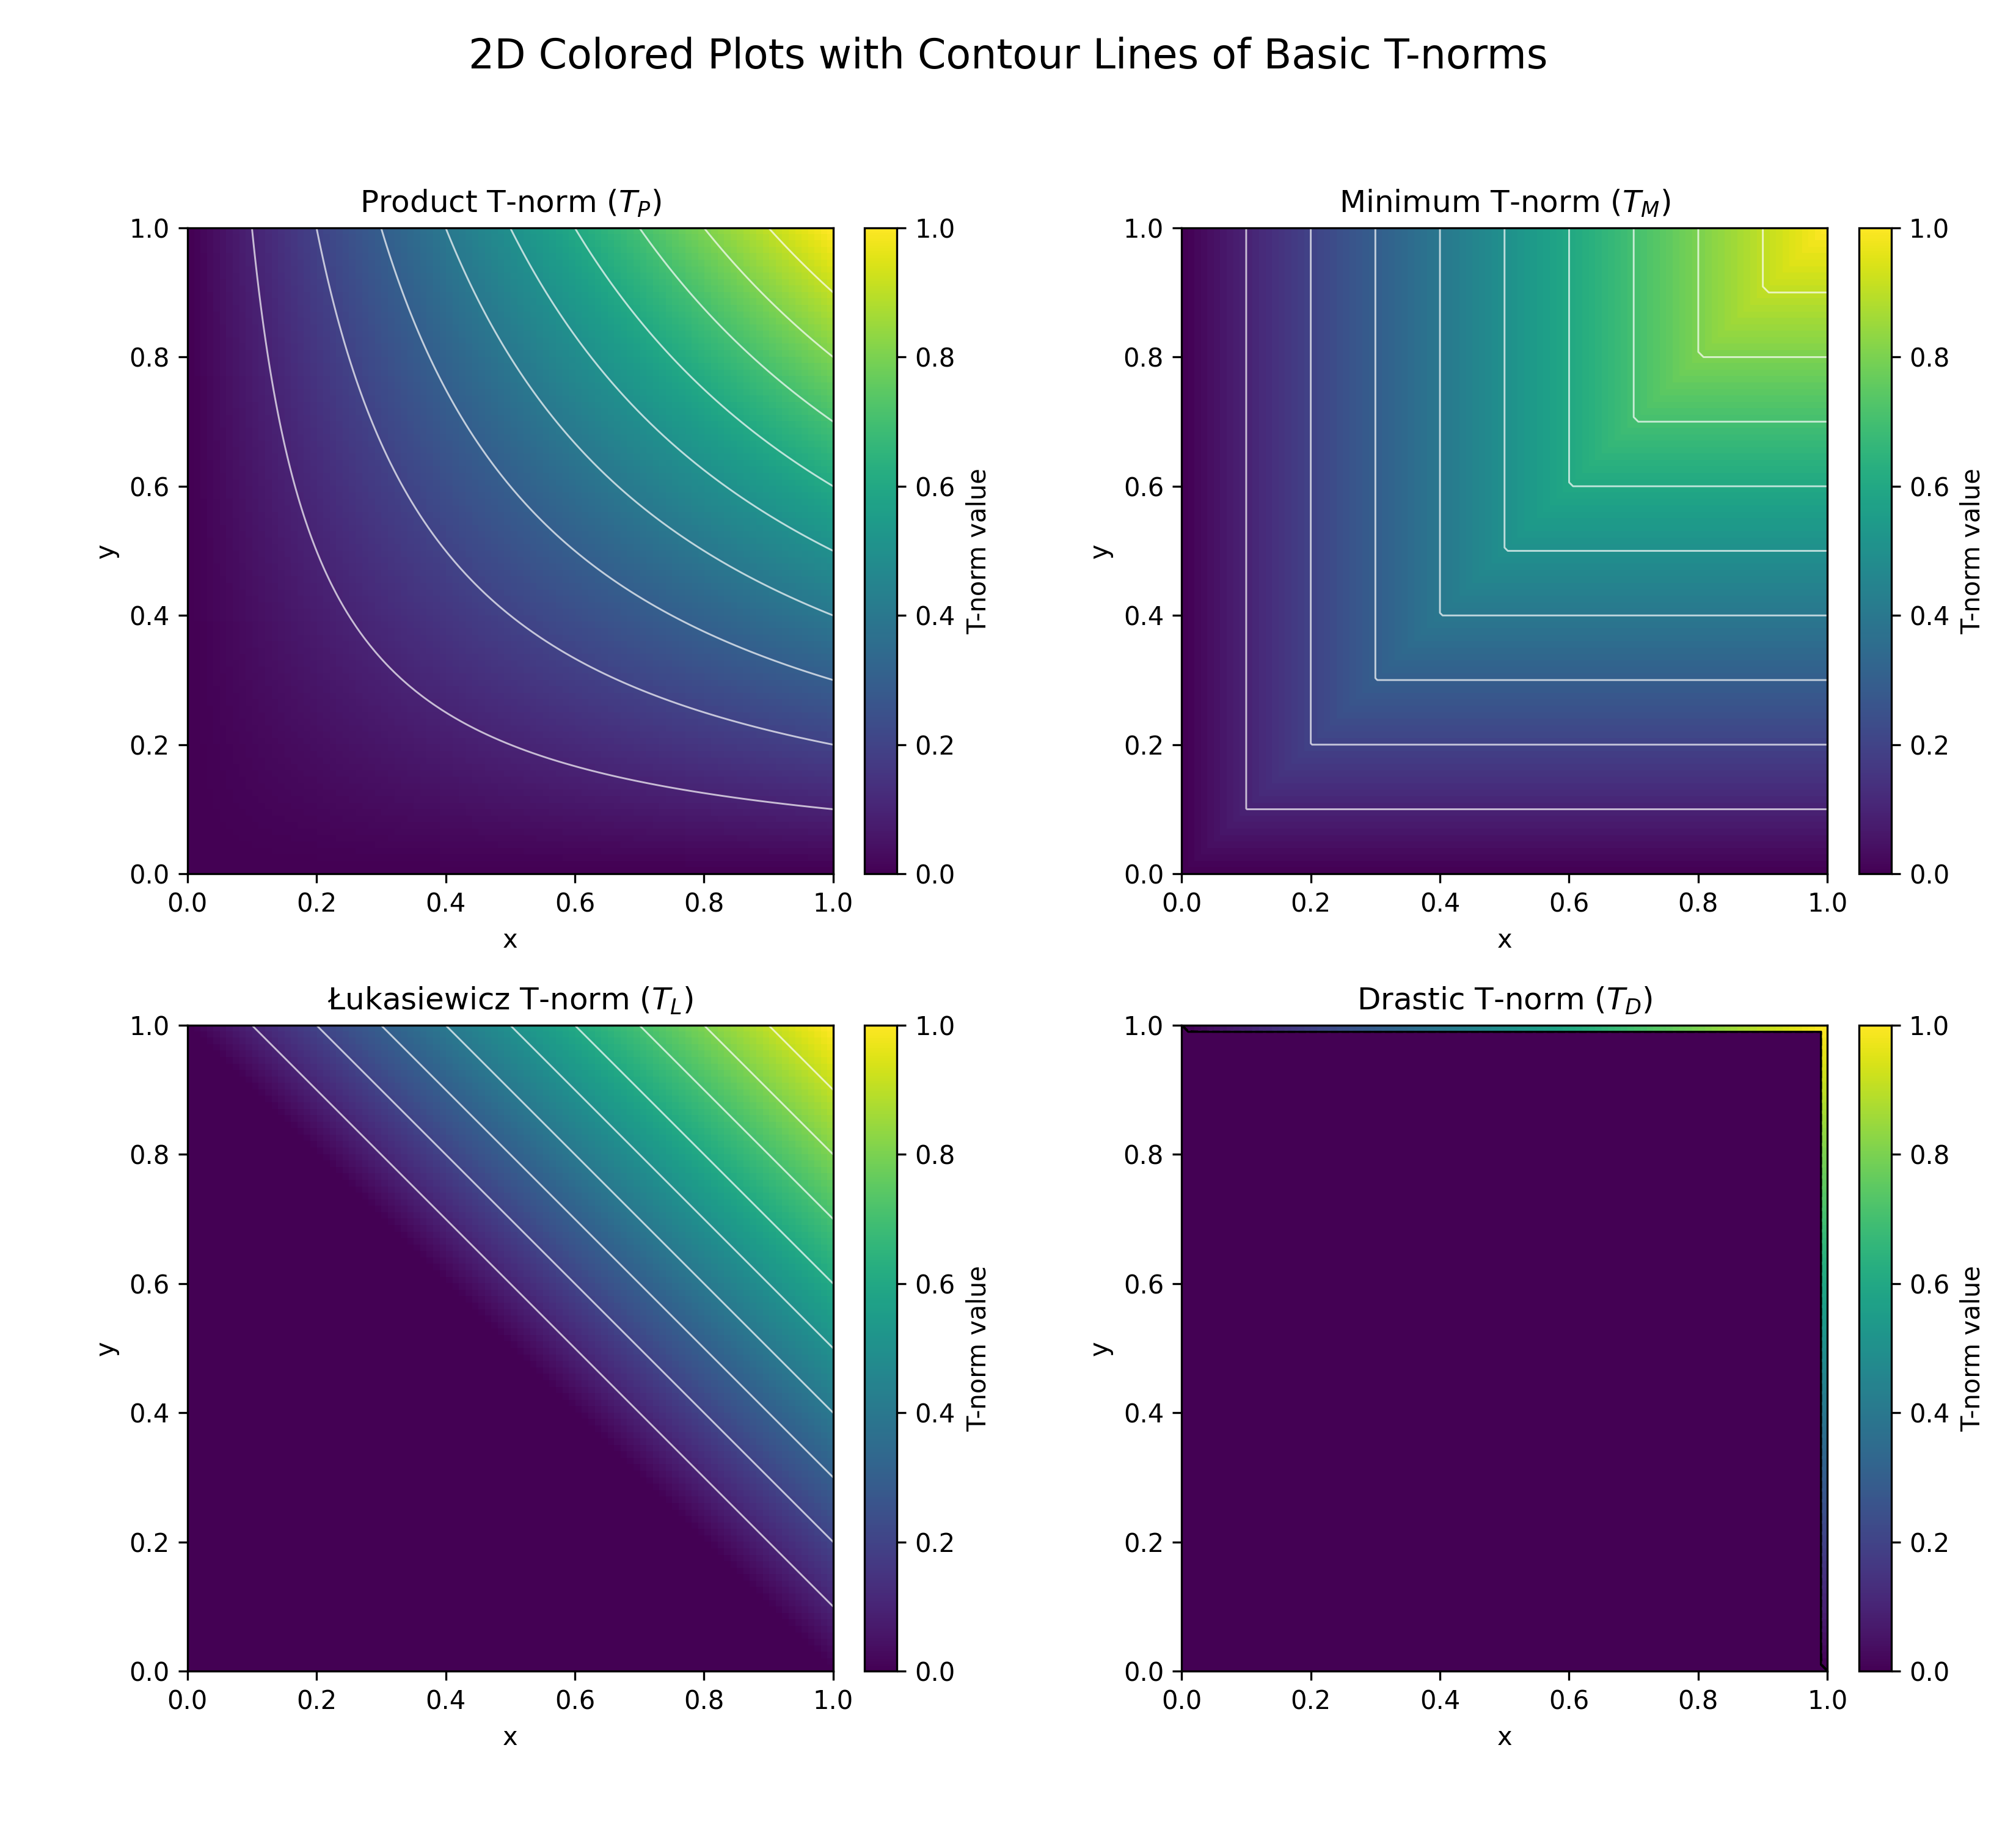
\includegraphics[width=0.85\textwidth]{ch1/figures/tnorms_2D_plots.png}
    \caption{Level curves of basic t-norms ($T_M$, $T_P$, $T_L$, $T_D$) in the unit square $[0,1]^2$. The different shapes of the white level curves illustrate the distinct behaviors and algebraic properties of each t-norm.}
    \label{fig:2D_tnorms}
\end{figure}


\begin{figure}[!ht]
    \centering
    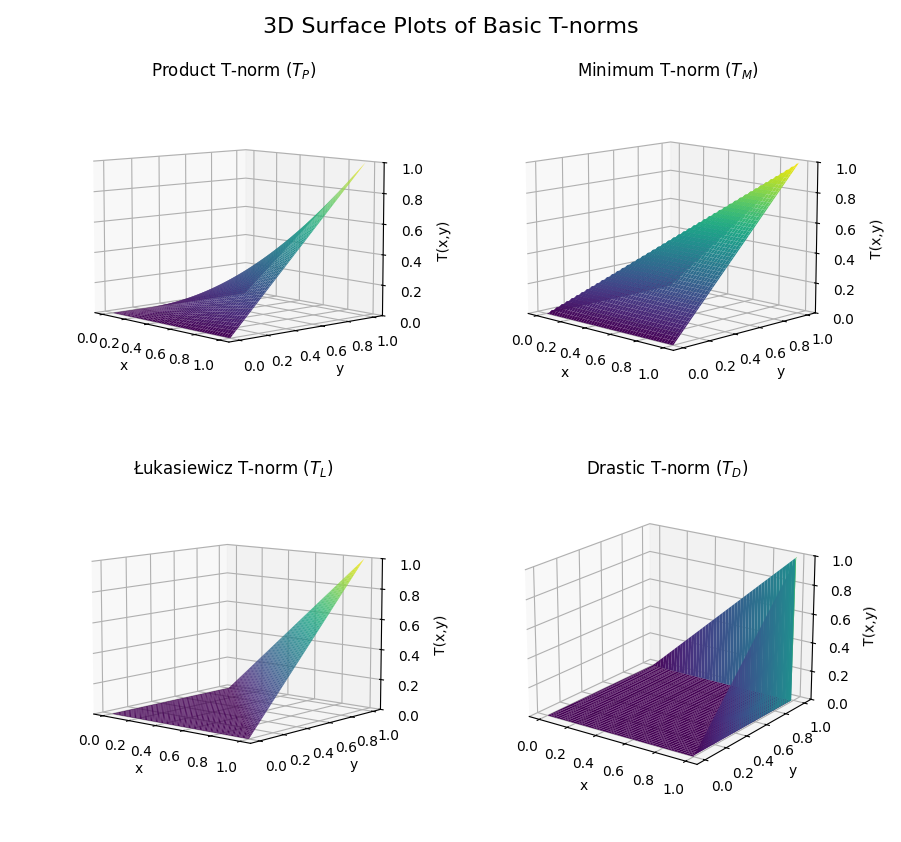
\includegraphics[width=0.95\textwidth]{ch1/figures/tnorms_3D_plots.png}
    \caption{3D surface plots of the basic t-norms ($T_M$, $T_P$, $T_L$, $T_D$) over the unit square $[0,1]^2$. The minimum t-norm forms a sharp ridge along $x=y$, the product t-norm is smoothly curved, the Łukasiewicz t-norm is planar except for a triangular region where it is zero, and the drastic t-norm is flat except for the edges. All of them are identical at the boundaries of the unit square.}
    \label{fig:tnorms_3D_plots}
\end{figure}


\subsection{Classification of T-norms}\label{sec:class_tnorms}
The first and most straight forward way to classify them is by defining the following partial order on the set of all t-norms. 
\begin{definition}[Weaker/Stronger t-norm {\cite[Def.~1.4]{Klement2000}}]\label{def:weaker}
  Given two t-norms $T_1$ and $T_2$, $T_1$ is said to be \emph{weaker} than $T_2$ (denoted $T_1 \leq T_2$) if $T_1(x,y) \leq T_2(x,y) \forall x,y \in [0,1]$.
  Equivalently, $T_2$ is said to be \emph{stronger} than $T_1$.
\end{definition}

\begin{remark}
  It's a fundamental result that for any t-norm $T$, we have $T_D \leq T \leq T_M$, where $T_D$ and $T_M$ are the drastic and the minimum t-norms respectively (\cite[Rem.~1.5]{Klement2000}).
\end{remark}

The interpretation is that a weaker t-norm can be seen as a stricter and more pessimistic intersection (conjunction in the fuzzy logic derived), returning lower membership values than a stronger one. Notice that it is not a total order: there are pairs of t-norms where none of them is weaker than the other. Some examples, such as the product $T_P$ and Yager $T_2^Y$ (see \ref{ex:families_tnorms} for the definition of the Yager family) t-norms, are shown in \cite[Fig.~6.1]{Klement2000}.\\


Another way to classify t-norms is based on their continuity properties. Continuous t-norms can be divided into two main classes (Fig.~\ref{fig:tnorm_classification}): Archimedean and non-Archimedean t-norms. The Archimedean t-norms can be further subdivided into strict and nilpotent t-norms (using the theorem \ref{thm:alg_arch_cont})\footnote{This classification is also characterized by the behavior of their generator functions at 0. For a more detailed discussion and definitions related to generators, see Appendix \ref{app:generators_tnorms}}:

\begin{itemize}
    \item $T$ is \textbf{strict} if it doesn't have any nilpotent elements except $0$. This means $T(x,y)>0$ whenever $x,y > 0$. (\cite[Cor.~3.30(i)]{Klement2000}).
    \item $T$ is \textbf{nilpotent} if every element in $]0,1[$ is nilpotent. This implies that for any $x,y \in ]0,1[$, there exists $n$ such that $T(x, \dots, x)$ ($n$ times) is $0$. (\cite[Cor.~3.30(ii)]{Klement2000}).
\end{itemize}


\begin{figure}[ht]
\centering
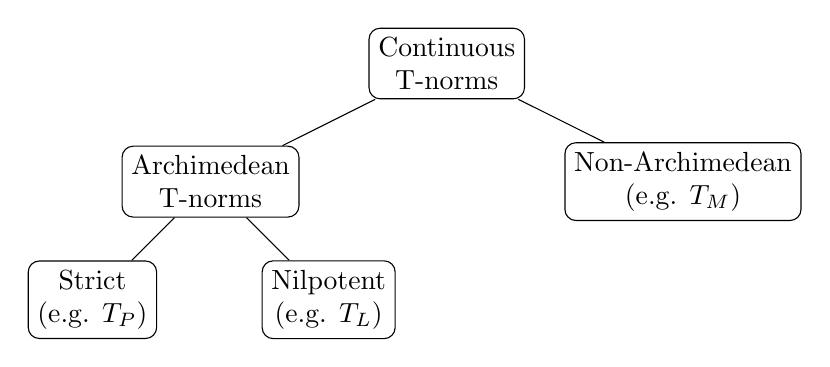
\begin{tikzpicture}[
    level 1/.style={sibling distance=60mm},
    level 2/.style={sibling distance=30mm},
    every node/.style={draw,rounded corners,align=center}
]
\node {Continuous\\ T-norms}
    child {
        node {Archimedean\\ T-norms}
        child {
            node {Strict\\ (e.g. $T_P$)}
        }
        child {
            node {Nilpotent\\ (e.g. $T_L$)}
        }
    }
    child {
        node {Non-Archimedean\\ (e.g. $T_M$)}
    };
\end{tikzpicture}
\caption{Classification of continuous t-norms}
\label{fig:tnorm_classification}
\end{figure}



Indeed, strict and nilpotent t-norms form two classes that are closed under certain isomorphic transformations: 

\begin{definition}[Isomorphic T-norms {\cite[Prop.~2.28(iv)]{Klement2000}}]
  Two t-norms $T_1$ and $T_2$ are \emph{isomorphic} if there exists a strictly increasing bijection $\varphi: [0,1] \to [0,1]$ (an automorphism of the unit interval) such that $T_2(x,y) = \varphi^{-1}(T_1(\varphi(x), \varphi(y)))$ for all $x,y \in [0,1]$.
\end{definition}
This definition is completely analogous for t-conorms. The isomorphism can be understood as a rescaling of the unit interval. The original t-norm is applied to this scaled domain and then the scale is reverted to make the output comparable to the original inputs $x,y$ (otherwise, the one identity property might not hold). Isomorphic t-norms share the same algebraic structure, merely operating on rescaled inputs and outputs via $\varphi$. A fundamental result is that (up to isomorphism) there are only two distinct types of continuous Archimedean t-norms: the product type and the Łukasiewicz type.
\begin{proposition}[{Classes of continuous Archimedean t-norms \cite[Cor.~5.7]{Klement2000}}]
  {\color{white}.}
  \begin{enumerate} 
      \item Every strict t-norm is isomorphic to the Product t-norm $T_P$.
      \item Every nilpotent t-norm is isomorphic to the Łukasiewicz t-norm $T_L$.
  \end{enumerate}
\end{proposition}

For general continuous t-norms that are not Archimedean, there must be non-trivial idempotent elements. These are constructed using ordinal sums.
\begin{definition}[Ordinal Sum of T-norms {\cite[Def.~3.44]{Klement2000}}]
Let $(T_\alpha)_{\alpha \in A}$ be a family of t-norms and $(]a_\alpha, e_\alpha[)_{\alpha \in A}$ be a family of non-empty, pairwise disjoint open subintervals of $[0,1]$. The t-norm $T$ defined by
\[
T(x,y) =
\begin{cases}
  a_\alpha + (e_\alpha - a_\alpha) \cdot T_\alpha \left( \frac{x-a_\alpha}{e_\alpha - a_\alpha}, \frac{y-a_\alpha}{e_\alpha - a_\alpha} \right) & \text{if } (x,y) \in [a_\alpha, e_\alpha]^2 \text{ for some } \alpha \in A \\
  \min(x,y) & \text{otherwise}
\end{cases}
\]
is called the \emph{ordinal sum} of the summands $(a_\alpha, e_\alpha, T_\alpha)$, $\alpha \in A$.
\end{definition}
Intuitively (see figure \ref{fig:ordinal_sum_tnorm}), an ordinal sum constructs a t-norm by combining scaled copies of other t-norms on the unit square $[0,1]^2$. For each interval $]a_\alpha, e_\alpha[$ along the main diagonal, a t-norm $T_\alpha$ operates within the square region $[a_\alpha, e_\alpha]^2$. Inside these "active" regions, inputs are first scaled down from $[a_\alpha, e_\alpha]$ to $[0,1]$ via linear transformations, then $T_\alpha$ is applied, and finally the result is scaled back to $[a_\alpha, e_\alpha]$. Outside these regions, the t-norm defaults to the minimum $T_M$, which ensures continuity (if the $T_\alpha$ are continuous) and makes the interval endpoints $a_\alpha, e_\alpha$ into idempotent elements of the resulting t-norm. This continuity at the boundaries of the active region is possible because any t-norm $T$ coincides with $T_M$ along the border of any square region centered in the diagonal $(x,x)$.\\

\begin{figure}[!ht]
    \centering
    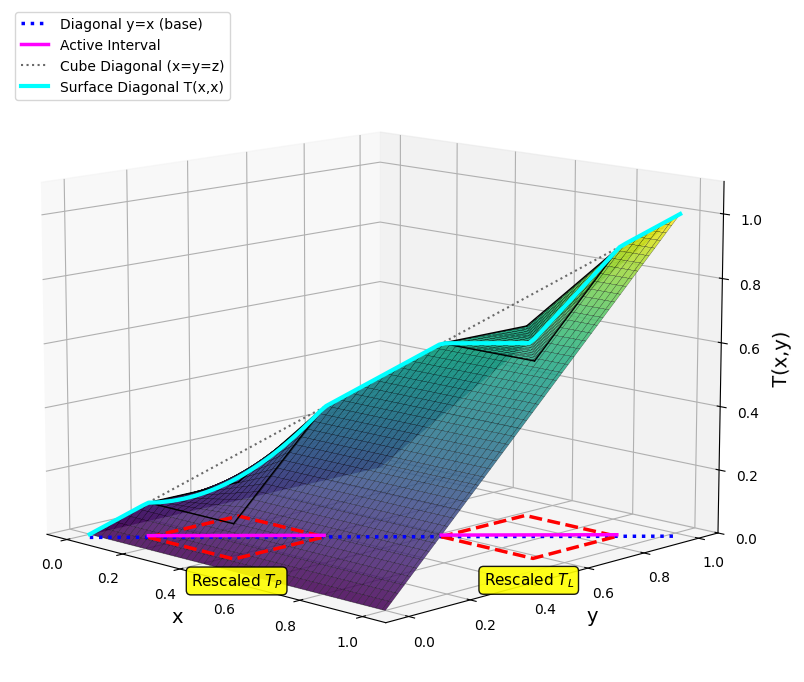
\includegraphics[width=0.9\textwidth]{ch1/figures/ordinal_sums.png}
    \caption{Visualization of an ordinal sum of t-norms. Each colored square (black on the surface, red on the xy plane) along the diagonal corresponds to an "active" region where a rescaled t-norm (Product or Łukasiewicz) operates. Outside these regions, the minimum t-norm $T_M$ is used. This illustrates how continuous t-norms can be built from Archimedean components via ordinal sums. It is inspired by \cite[Fig.~3.16]{Klement2000}}
    \label{fig:ordinal_sum_tnorm}
\end{figure}



\begin{theorem}[Representation of Continuous T-norms {\cite[Thm.~5.11]{Klement2000}}]
  A function $T: [0,1]^2 \to [0,1]$ is a continuous t-norm if and only if $T$ is uniquely representable as an ordinal sum of continuous Archimedean t-norms.
\end{theorem}

The main idea behind this representation is leveraging the idempotent elements in the diagonal. Start with all the diagonal being idempotent (only possibility is $T_M$), and remove all the non-idempotent intervals (where the t-norm is locally Archimedean) with one of the two possibilities in the continuous case: strict (isomorphic to $T_P$) or nilpotent (isomorphic to $T_L$).

\begin{remark}
  If the family of subintervals is empty, the ordinal sum is defined as $T_M$.
\end{remark}

Unlike continuous t-norms, non-continuous t-norms generally lack a unifying framework based on generator functions that allows for a similar classification. Their analysis, therefore, focuses on the particular (semi-)continuity and algebraic characteristics. For examples and a discussion on semi-continuity of t-norms, see appendix \ref{app:cont_tnorms} and \ref{app:semicont-tnorms}.










































